\documentclass{article}
\usepackage{amsmath, amssymb, cite, algorithmic, url, braket}
\usepackage{graphicx}
\usepackage{pythonhighlight}
\usepackage[margin=1.5cm]{geometry}
\usepackage[title]{appendix}
\usepackage{listings}

\graphicspath{{../pic/}}
\lstset{
language=[ANSI]{C},
showtabs=true,
tab=,
tabsize=2,
basicstyle=\ttfamily\footnotesize,%\setstretch{.5},
stringstyle=\color{stringcolour},
showstringspaces=false,
alsoletter={1234567890},
otherkeywords={\%, \}, \{, \&, \|},
keywordstyle=\color{keywordcolour}\bfseries,
upquote=true,
morecomment=[s]{/*}{*/},
commentstyle=\color{commentcolour}\slshape,
literate=*%
{=}{{\literatecolour=}}{1}%
{-}{{\literatecolour-}}{1}%
{+}{{\literatecolour+}}{1}%
{*}{{\literatecolour*}}{1}%
{!}{{\literatecolour!}}{1}%
{[}{{\literatecolour[}}{1}%
{]}{{\literatecolour]}}{1}%
{<}{{\literatecolour<}}{1}%
{>}{{\literatecolour>}}{1}%
% {>>>}{\pythonprompt}{3}%
,%
frame=trbl,
rulecolor=\color{black!40},
backgroundcolor=\color{white},
breakindent=.5\textwidth,frame=single,breaklines=true
}

\begin{document}
\title{DSP Homework 02}
\author{Xu, Minhuan}
\maketitle
\tableofcontents

\begin{abstract}
    \subsubsection*{Problem 1}
    This week, we watched 2 videos about chip making and a new black hole picture. First, in watching the video of chip making, I went through the knowledge of how the silicon become doped semiconductor, and eventually is changed into MOSFETs which is the basic unit of out complex chips. Second, the video of black hole introduced how we can take the photo of the second black hole with the help of a large system called EHT.

    \subsubsection*{Problem 2}

    The cells who distinguish colors are called cones, and people who have 3-color vision have 3 kinds of them. Each of them can see about 100 levels of colors, so at all we can see $1,000,000$.

    \subsubsection*{Problem 3}

    I trid to find out whoever did the research of mood sampling in a day, but failed. So, I turn to some pratical experiments and find out that people's (as a group) highest frequency at which they can change their mood is about $2\sim 3 ~ \mathrm{times/day}$, so I think in this situation, we can set the frequency of sampling to $6~\mathrm{times/day}$.

    \subsubsection*{Problem 4}

    The proposal is about how to do the sound processing and what the Hi-fi is. Why I want to do a research like this is I doubt of the necessity of expensive devices in daily music appreciation.


\end{abstract}

\section{Problem 1}
\subsection{Problem Restatement}

Write a summary of this week’s video(s) and your further thoughts on the content.

\subsection{Summary and My thoughts}
\subsubsection{Chip Making}

This video shows us in detail how a small chip is born from silicon in the sand. First of all, silicon is a semiconductor, which does not contain the free electrons or holes, so it cannot behave like what we need. So we use the so-called dopants of boron and phosphorus, which are near silicon in the periodic table of elements and are non-metallic elements to make the mixture have free electrons or holes, so as to form p-type or n-type semiconductors, and then make the unidirectional conductive PN junction.

With the PN junction, we can make BJT or MOSFET. The MOSFET is by far the most common transistor in digital circuits, as billions may be included in a memory chip or microprocessor.\cite{enwiki:1109379174} How MOSFETs work can be described as: a high level or a low level is applied to the grid. At this time, the voltage applied between the drain and the source can form the corresponding doped conductive channel in the tube to successfully form the current, rather than being limited by the reverse conducting PN junction.

With the development of digital circuits and its logic design, we can theoretically construct a chip's design chart, and what we need to do is to make it.

What is shown in the video is that people in the chip factory finally make a large chip board through complex processes in a clean room, and finally get small chips through encapsulation.

After watching this video, I can understand how the chips are theoretically constructed. But, I can barely understand the process that how the chips are manufactured in the clean room, so I guess it's just too complex. 

However, we will need more and more chips like those mentioned in this video, which means more effort should be made in the future.

\subsubsection{New Black Hole Photo}

An international team of astronomers led by scientists at the Center for Astrophysics | Harvard \& Smithsonian who produced the first direct image of a black hole three years ago have now produced a portrait of a second, this time a much-anticipated glimpse of one at the heart of the Milky Way.\cite{second-black-hole-image}

And this video is about this news about our second capture of the trace of black holes, thus further promoting our understanding and research.

First, the significance of taking this photo is that we can understand more clearly that the object in the first photo is indeed a black hole, and the appearance of a black hole in our observation has been further confirmed.

Secondly, through theoretical confirmation, if we want to take this black hole picture with a telescope, its diameter must be at least at the level of the earth's radius, so we adopted the EHT. 

By linking together existing telescopes using new systems, the EHT creates a fundamentally new instrument with angular resolving power that is the highest possible from the surface of the Earth.

\section{Problem 2}

\subsection{Problem Restatement}

Find a way to determine how many different colors your eyes can see.

\subsection{Solution}

Colors refer to the frequency of the light wave which is kind of electromagnetic wave. But not all frequency bands of electromagnetic waves can be perceived by the eyes, and the frequency range of visible light is about $830 - 750~\mathrm{THz} ~\sim ~ 395 - 360 ~\mathrm{THz}$.

So, the first thing we should do is to find out how our eyes receive and distinguish the colors. Humans normally have three types of cones, usually designated L, M and S for long, medium and short wavelengths respectively.\cite{enwiki:1107424454} The three types of cones cannot distinguish every single color, there always are two color that are too close to tell. So I guess there are many bands which cones can receive, and colors in one band can only be interpreted to certain color in this band, like we all do in sampling and quantification.

Then, we should find out the smallest difference which our eyes can tell---so-call the bandwidth. Here comes the problem, we can't make sure whether the bands are linearly placed in all frequency, so a detailed experiment is required. In this experiment, we need only one kind of cones can receive the light --- Perhaps we can use only short wavelengths light to test the S cones. I don't know whether this works, but I want to continue my thought experiment--- then choose hundreds of lights, let the participants tell the difference between two colors in an area while narrowing the gap of frequency until he or she cannot distinguish, and go to another area. So we can calculate how many colors can people distinguish in one area, and after adding them all, we will get the number that one kind of cones can tell. The number our eyes can distinguish is the 3rd power of that number.

Through searching on the Internet, I know that 100 is the most colors we can see with one kind of cones. So, at all we can see 1,000,000 of colors with our eyes.

\section{Problem 3}

\subsection{Problem Restatement}
In general a person’s mood changes continuously in a day. Determine the right uniform sampling period $T$ of a person’s
mood in a day so that virtually no information is lost after sampling.

\subsection{Solution}
Please allow me to cite a long paragraph below to indicate my opinion.

"Individual mood is an affective state that is important for physical and emotional well-being, working memory, creativity, decision-making, and immune response. Mood is influenced by levels of dopamine, serotonin, and other neurochemicals, as well as by levels of hormones. Mood is also externally modified by social activity, such as daily routines of work, commuting, and eating. Because of this complexity, accurate measurement of affective rhythms at the individual level has proven elusive." \cite{mood_sci}

I am doubting whether we can truely determine the \emph{right} period of someone's mood in a day. It is changing every moment. Considering the reaction time of human is about $0.7~s$, maybe the mood can change in only 2 seconds, but it also can remain high or down for a whole day, even a whole week. I cannot prove myself, but I have a guess that the \emph{possible} uniform sampling period $T$ should be $2 \sim 3~s$. That's the shortest time I can imagine for one's mood changes.

However, during searching for information, I found some articles has found out the rough wave of people's mood, see fig.\ref{fig1} \cite{mood_sci}. Their research almost rely on the API of social media, which means the result can only represent those who are using the social media. And, this is a group, not an individual.

\begin{figure}[htbp]
    \centering
    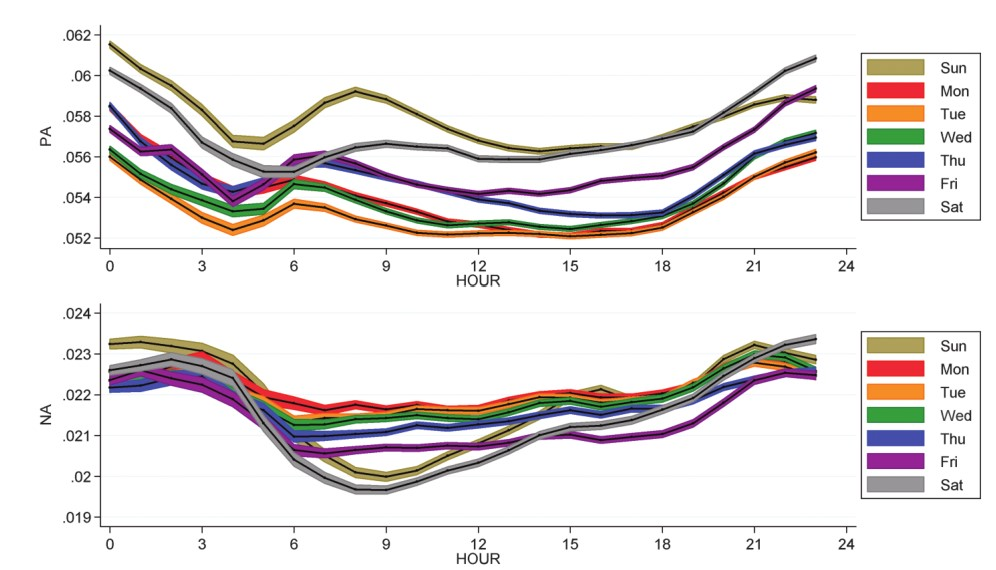
\includegraphics[keepaspectratio,width=300pt]{mood_in_a_day.jpg}
    \caption{Hourly changes in individual affect}\label{fig1}
\end{figure}

What we can find in this figure is that the line charts of statistical results have most 4 extreme points in a day. Then, we can suppose the highest frequency at which people can largely change their mood is $2\sim 3 ~ \mathrm{times/day}$. Finally, in my opinion, the sampling period can be set to $6~\mathrm{times/day}$.

\section{Problem 4}
\subsection{Problem Restatement}
Write your first monthly project proposal.

\subsection{My Proposal}

First of all, I will explore how the sound information starts from the vibration of the vocal cords, goes to our speakers in terms of theory and hardware, and finally allows the listener to receive the information.

Then, I will purposely explore whether expensive devices on the market are necessary in daily music appreciation from sampling, DAC, power amplification and other aspects, and why major music platforms emphasize the concept of 'lossless music file format' such as 'FLAC'.

Finally, the reason for this proposal is that I have learned about the above-mentioned devices without any knowledge of electronic engineering and purchased some of the hardware without understanding the principle. I will introduce my current desktop audio solution in the article and evaluate it with my newly acquired knowledge.

% \bibliographystyle{ieeetr}
% \bibliography{../bib/database}

\begin{appendices}
    
\end{appendices}

\end{document}

